\documentclass[11pt,a4paper]{report}
\usepackage[utf8]{inputenc}
\usepackage[T1]{fontenc}
\usepackage{geometry}
\geometry{top=2.2cm,bottom=2.2cm,left=2.2cm,right=2.2cm}
\usepackage{amsmath,amssymb}
\usepackage{xcolor}
\usepackage{booktabs}
\usepackage{tabularx}
\usepackage{fancyhdr}
\usepackage{enumitem}
\usepackage{listings}
\usepackage{tikz}
\usetikzlibrary{shapes.geometric,arrows.meta,positioning,fit,backgrounds,calc,decorations.pathreplacing}
\usepackage{hyperref}
\usepackage{titlesec}

% Paleta de Colores Corporativa
\definecolor{brandNavy}{RGB}{15, 32, 67}
\definecolor{brandBlue}{RGB}{24, 90, 188}
\definecolor{brandTeal}{RGB}{0, 150, 166}
\definecolor{brandGreen}{RGB}{34, 139, 34}
\definecolor{brandRed}{RGB}{178, 34, 34}
\definecolor{codeBg}{RGB}{248, 249, 251}
\definecolor{codeBorder}{RGB}{220, 224, 230}
\definecolor{textDark}{RGB}{30, 41, 59}

% Configuración de Hipervínculos
\hypersetup{
    colorlinks=true,
    linkcolor=brandBlue,
    filecolor=brandTeal,
    urlcolor=brandBlue,
    pdftitle={Feature Book: AgentIA Enterprise Microservice Generator},
    pdfauthor={AgentIA Architecture Team}
}

% Configuración de Encabezados y Pies de Página
\pagestyle{fancy}
\fancyhf{}
\fancyhead[L]{\textcolor{brandNavy}{\textbf{AgentIA}} $\cdot$ \textit{Feature Book \& Arquitectura}}
\fancyhead[R]{\textcolor{gray}{\thepage}}
\fancyfoot[C]{\textcolor{gray}{\footnotesize AgentIA Enterprise $\cdot$ Scaffolding Determinista, P-Stack \& OpenShip Local Cloud}}
\renewcommand{\headrulewidth}{0.5pt}
\renewcommand{\footrulewidth}{0.3pt}

% Configuración de listings para Java y JSON
\lstset{
    backgroundcolor=\color{codeBg},
    basicstyle=\ttfamily\footnotesize\color{textDark},
    breaklines=true,
    breakatwhitespace=true,
    captionpos=b,
    commentstyle=\color{gray}\textit,
    frame=single,
    framerule=0.5pt,
    rulecolor=\color{codeBorder},
    keywordstyle=\color{brandBlue}\bfseries,
    stringstyle=\color{brandTeal},
    numberstyle=\tiny\color{gray},
    numbers=left,
    numbersep=7pt,
    showstringspaces=false,
    tabsize=2
}

% Formato de Títulos
\titleformat{\chapter}[display]
  {\normalfont\bfseries\color{brandNavy}}
  {\filleft\Huge\textbf{\color{brandTeal}Capítulo \thechapter}}
  {1ex}
  {\titlerule\vspace{1ex}\huge}
  [\vspace{1ex}\titlerule]

\titleformat{\section}
  {\normalfont\Large\bfseries\color{brandNavy}}
  {\thesection}{1em}{}

\titleformat{\subsection}
  {\normalfont\large\bfseries\color{brandBlue}}
  {\thesubsection}{1em}{}

\begin{document}

% --- PORTADA ---
\begin{titlepage}
    \centering
    \vspace*{1.5cm}
    
    {\Huge \textbf{\color{brandNavy}AgentIA Enterprise Microservice Generator}}\\[0.6cm]
    {\LARGE \textbf{\color{brandTeal}Libro Integral de Características y Arquitectura}}\\[0.4cm]
    {\large \textit{Orquestación con LangGraph, Scaffolding Determinista, Reparación Quirúrgica P-Stack y Despliegue en OpenShip}}\\[1.5cm]
    
    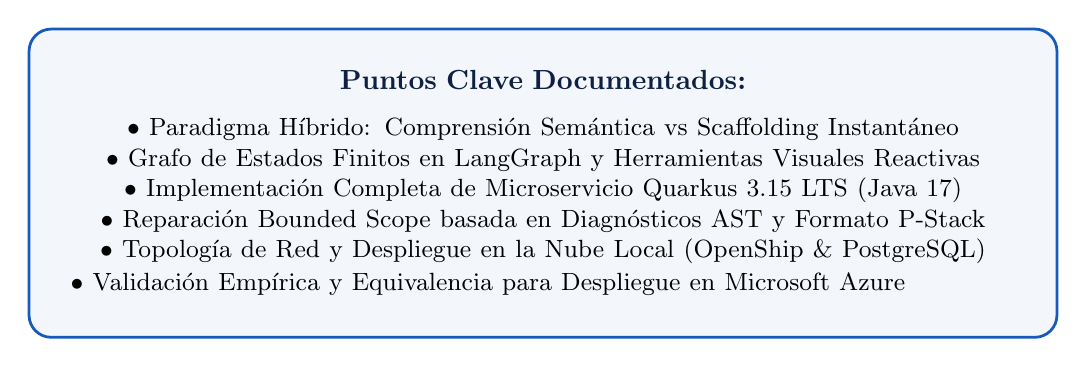
\begin{tikzpicture}
        \node[draw=brandBlue, fill=brandBlue!5, rounded corners=8pt, line width=1pt, inner sep=15pt, text width=12cm] {
            \centering
            \textbf{\color{brandNavy}Puntos Clave Documentados:}\\[0.2cm]
            \small
            $\bullet$ Paradigma Híbrido: Comprensión Semántica vs Scaffolding Instantáneo\\
            $\bullet$ Grafo de Estados Finitos en LangGraph y Herramientas Visuales Reactivas\\
            $\bullet$ Implementación Completa de Microservicio Quarkus 3.15 LTS (Java 17)\\
            $\bullet$ Reparación Bounded Scope basada en Diagnósticos AST y Formato P-Stack\\
            $\bullet$ Topología de Red y Despliegue en la Nube Local (OpenShip \& PostgreSQL)\\
            $\bullet$ Validación Empírica y Equivalencia para Despliegue en Microsoft Azure
        };
    \end{tikzpicture}
    
    \vfill
    
    \begin{tabular}{ll}
        \textbf{Versión del Sistema:} & 2.4.0-Enterprise \\
        \textbf{Framework Base:} & Quarkus 3.15.0 LTS (Jakarta EE 10 / Java 17) \\
        \textbf{Motor de Orquestación:} & LangGraph State Machine con P-Stack Repair Loop \\
        \textbf{Fecha de Publicación:} & Octubre 2026 \\
        \textbf{Estado de Auditoría:} & Verificado y Aprobado con OpenShip \\
    \end{tabular}
    
    \vspace*{1cm}
\end{titlepage}

% --- TABLA DE CONTENIDOS ---
\tableofcontents
\newpage

% --- CAPÍTULO 1 ---
\chapter{Visión General y Herramientas Visuales}

\section{Introducción y Misión}
La plataforma \textbf{AgentIA} representa un cambio de paradigma en la ingeniería asistida por inteligencia artificial para microservicios empresariales. A diferencia de los generadores de código tradicionales basados en prompts no estructurados (que sufren de latencia inaceptable, alto coste de tokens y alucinaciones frecuentes en dependencias de Maven), AgentIA implementa una arquitectura \textbf{híbrida y reactiva}.

\section{Herramientas Visuales Integradas en el Ecosistema}
Para evitar que el proceso sea una ``caja negra'', el sistema integra herramientas de inspección en dos niveles:

\subsection{1. Visualizadores de la Interfaz de Usuario (AgentIA Studio)}
\begin{itemize}[leftmargin=1.5cm]
    \item \textbf{LangGraph State Visualizer (\texttt{LangGraphStateVisualizer.tsx}):} Proyecta en vivo el estado del grafo de ejecución con badges reactivos (\texttt{SUCCESS}, \texttt{RUNNING}, \texttt{ERROR}, \texttt{NO\_FIX}), transiciones de aristas y un contador de iteraciones acotadas ($k \in [0, 3]$).
    \item \textbf{Terminal ANSI en Tiempo Real (\texttt{RealtimeTerminal.tsx}):} Canaliza la salida de los comandos de Maven (\texttt{mvn test-compile}) y Docker mediante streaming continuo, resaltando advertencias del compilador y stack traces.
    \item \textbf{Cajón de Reparación Quirúrgica (\texttt{ExecutionDrawer.tsx}):} Permite al desarrollador inspeccionar el árbol de diagnósticos del AST de Java y revisar el parche diff unificado antes de su aplicación en disco.
\end{itemize}

\subsection{2. Entorno Visual de la Nube Local (OpenShip Dashboard)}
Permite gestionar y visualizar la topología de contenedores en tiempo de ejecución:
\begin{itemize}[leftmargin=1.5cm]
    \item \textbf{Monitor de Servicios:} Estado de salud del contenedor Quarkus (\texttt{/q/health}) y PostgreSQL.
    \item \textbf{Swagger UI Interactivo:} Explorador de contratos OpenAPI accesible en \texttt{http://localhost:8080/q/swagger-ui}.
    \item \textbf{Consola de Red:} Mapeo de la red virtual de puente (\texttt{openship\_net}) y flujos de tráfico TCP.
\end{itemize}

\newpage

% --- CAPÍTULO 2 ---
\chapter{Arquitectura del Sistema y Flujo de Orquestación}

\section{El Paradigma Híbrido: Tokens Eficientes vs Boilerplate}
La premisa central de diseño, alineada con las directrices del Líder Técnico, establece:
\begin{quote}
\textit{``No se deben quemar tokens de LLM en código repetitivo y determinista que un arquetipo estructurado resuelve en milisegundos. El LLM debe reservarse para el razonamiento de negocio y la corrección quirúrgica.''}
\end{quote}

Matemáticamente, el ahorro de tokens de salida ($\Delta T$) frente al enfoque ingenuo se modela como:
\begin{equation}
\Delta T = T_{\text{naive}} - T_{\text{hybrid}} = \sum_{i=1}^{M} L(F_i) - 0 \approx \mathcal{O}(N_{\text{entidades}} \cdot 1,800 \text{ tokens})
\end{equation}
donde $L(F_i)$ es la longitud en tokens del archivo $i$ generado mediante plantillas Jinja2 deterministas auditadas.

\section{Grafo de Estados Finitos en LangGraph}
El orquestador modela el ciclo de vida del microservicio como una máquina de estados:
\begin{equation}
\mathcal{M} = \langle \mathcal{S}, \Sigma, \mathcal{T}, s_0, \mathcal{F} \rangle
\end{equation}
donde:
\begin{itemize}
    \item $\mathcal{S} = \{\text{Validate}, \text{Generate}, \text{Verify}, \text{Repair}, \text{Terminal}\}$
    \item $\Sigma = \{\text{ValidSpec}, \text{ScaffoldOK}, \text{BuildPass}, \text{BuildFail}, \text{Patched}, \text{MaxAttemptsExceeded}\}$
    \item $\mathcal{T}: \mathcal{S} \times \Sigma \to \mathcal{S}$ define la función de transición de estados.
\end{itemize}

\begin{figure}[h!]
\centering
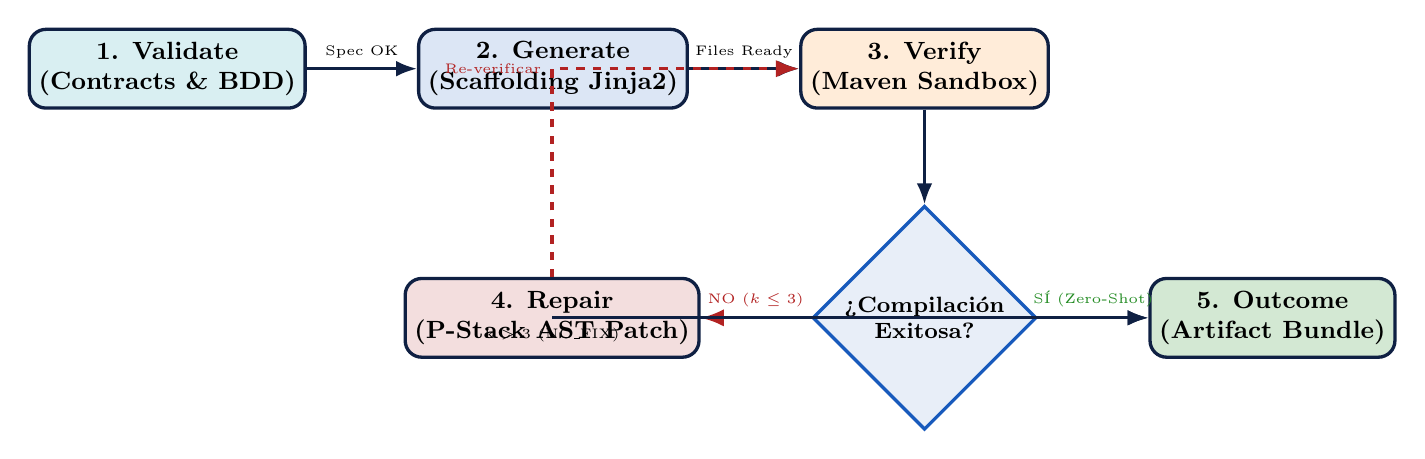
\begin{tikzpicture}[
    node distance=1.8cm and 1.4cm,
    state/.style={rectangle, rounded corners=6pt, draw=brandNavy, line width=1.2pt, fill=codeBg, minimum width=2.4cm, minimum height=1cm, align=center, font=\small\bfseries},
    decision/.style={diamond, draw=brandBlue, line width=1.2pt, fill=brandBlue!10, inner sep=2pt, font=\footnotesize\bfseries, align=center},
    edge/.style={-Latex, line width=1pt, draw=brandNavy},
    repedge/.style={-Latex, line width=1.2pt, draw=brandRed, dashed}
]

% Nodos
\node[state, fill=brandTeal!15] (val) {1. Validate\\(Contracts \& BDD)};
\node[state, fill=brandBlue!15, right=of val] (gen) {2. Generate\\(Scaffolding Jinja2)};
\node[state, fill=orange!15, right=of gen] (ver) {3. Verify\\(Maven Sandbox)};
\node[decision, below=1.2cm of ver] (check) {¿Compilación\\Exitosa?};
\node[state, fill=brandRed!15, left=of check] (rep) {4. Repair\\(P-Stack AST Patch)};
\node[state, fill=brandGreen!20, right=of check] (term) {5. Outcome\\(Artifact Bundle)};

% Aristas
\draw[edge] (val) -- node[above, font=\tiny] {Spec OK} (gen);
\draw[edge] (gen) -- node[above, font=\tiny] {Files Ready} (ver);
\draw[edge] (ver) -- (check);
\draw[edge] (check) -- node[above, font=\tiny\color{brandGreen}] {SÍ (Zero-Shot)} (term);
\draw[repedge] (check) -- node[above, font=\tiny\color{brandRed}] {NO ($k \le 3$)} (rep);
\draw[repedge] (rep) |- node[left, font=\tiny\color{brandRed}] {Re-verificar} (ver);
\draw[edge] (rep) |- node[below, font=\tiny] {k > 3 (NO\_FIX)} (term);

\end{tikzpicture}
\caption{Diagrama de Flujo del Orquestador LangGraph con Bucle de Reparación Acotado.}
\label{fig:langgraph}
\end{figure}

\section{Explicación Detallada de Cada Nodo}
\begin{enumerate}[leftmargin=1.5cm]
    \item \textbf{Nodo Validate (\texttt{validate\_node}):} Evalúa la coherencia semántica del Blueprint: existencia de claves primarias, formatos de paquetes Java estándar (\texttt{com.banco.*}) y escenarios de prueba Gherkin válidos.
    \item \textbf{Nodo Generate (\texttt{generate\_node}):} Lee el Blueprint normalizado e instancia dinámicamente las plantillas del arquetipo Quarkus 3.15 LTS (Entidades Panache, Repositorios, Recursos JAX-RS, \texttt{pom.xml}, \texttt{application.properties} y \texttt{Dockerfile}).
    \item \textbf{Nodo Verify (\texttt{verify\_node}):} Ejecuta un runner hermético (\texttt{LocalDockerRunner} o \texttt{LocalSubprocessRunner}) lanzando \texttt{mvn -B test-compile}. Si la compilación falla, un parser regex convierte los errores de \texttt{javac} en objetos tipados \texttt{DiagnosticIssue}.
    \item \textbf{Nodo Repair (\texttt{repair\_node}):} Si existen fallas, extrae el archivo afectado, localiza la línea del AST y le solicita al LLM un parche quirúrgico en formato de bloque de búsqueda y reemplazo.
    \item \textbf{Nodo Terminal (\texttt{terminal\_node}):} Consolida los metadatos de ejecución, genera el paquete final y registra la traza en la base de datos de auditoría.
\end{enumerate}

\newpage

% --- CAPÍTULO 3 ---
\chapter{El Principio P-Stack y Reglas de la Constitución}

\section{¿Qué es P-Stack?}
\textbf{P-Stack} (Prompt/Patch Stack) es el estándar de ingeniería que rige las operaciones de modificación de código por parte de agentes inteligentes. En lugar de permitir reescrituras globales, P-Stack exige la emisión de bloques atómicos delimitados:

\begin{lstlisting}[language=Java, caption={Ejemplo de Parche P-Stack con Bloques SEARCH/REPLACE}]
<<<<<<< SEARCH
    @GET
    @Path("/estado/{estado}")
    public List<IniciacionPago> listarPorEstado(@PathParam("estado") String estado) {
        return repository.list("estado", estado);
    }
=======
    @GET
    @Path("/estado/{estado}")
    public List<IniciacionPago> listarPorEstado(@PathParam("estado") String estado) {
        return repository.findByEstado(estado);
    }
>>>>>>> REPLACE
\end{lstlisting}

\section{Bounded Surgical Scope (Principio de la Constitución)}
Tal como se implementa en \texttt{app/orchestrator/execution\_nodes.py}, el agente de reparación tiene su radio de acción delimitado de forma estricta:
\begin{equation}
\mathcal{A}_{\text{permitidos}} = \{ f \in \mathcal{F}_{\text{workspace}} \mid \exists \, \delta \in \text{Diagnostics} \text{ tal que } \text{file}(\delta) = f \}
\end{equation}

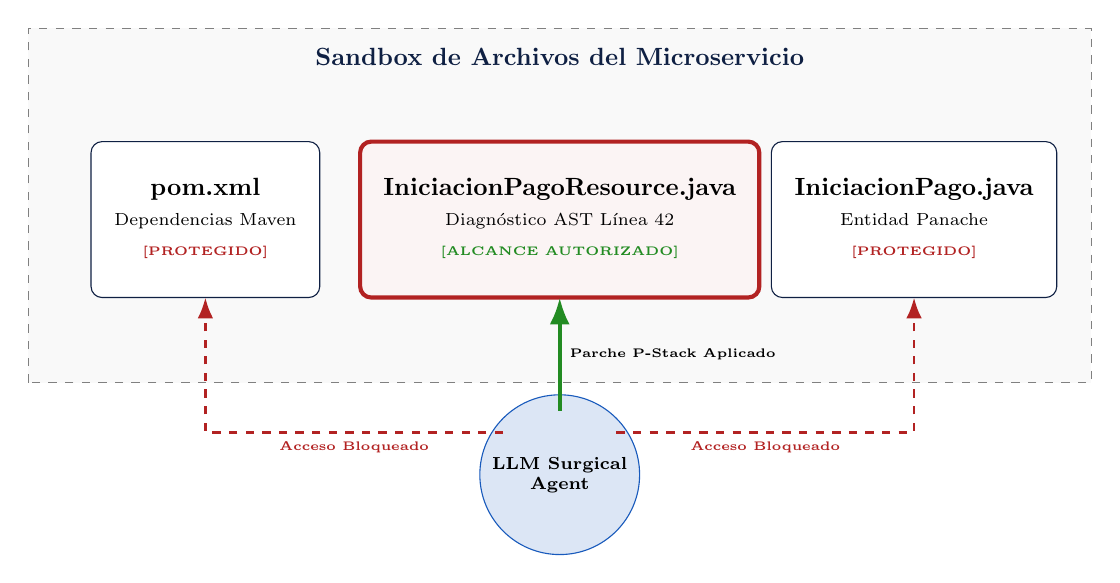
\begin{tikzpicture}[scale=0.9, every node/.style={transform shape}]
    % Entorno
    \draw[dashed, fill=gray!5, draw=gray] (-0.5,-0.5) rectangle (14.5,4.5);
    \node at (7, 4.1) {\textbf{\color{brandNavy}Sandbox de Archivos del Microservicio}};

    % Archivo intocable
    \node[draw=brandNavy, fill=white, rounded corners, minimum width=3.2cm, minimum height=2.2cm] at (2, 1.8) {
        \begin{tabular}{c}
            \textbf{pom.xml}\\
            \scriptsize Dependencias Maven\\
            \tiny \color{brandRed}\textbf{[PROTEGIDO]}
        \end{tabular}
    };

    % Archivo con error
    \node[draw=brandRed, line width=1.5pt, fill=brandRed!5, rounded corners, minimum width=3.8cm, minimum height=2.2cm] at (7, 1.8) {
        \begin{tabular}{c}
            \textbf{IniciacionPagoResource.java}\\
            \scriptsize Diagnóstico AST Línea 42\\
            \tiny \color{brandGreen}\textbf{[ALCANCE AUTORIZADO]}
        \end{tabular}
    };

    % Archivo no afectado
    \node[draw=brandNavy, fill=white, rounded corners, minimum width=3.2cm, minimum height=2.2cm] at (12, 1.8) {
        \begin{tabular}{c}
            \textbf{IniciacionPago.java}\\
            \scriptsize Entidad Panache\\
            \tiny \color{brandRed}\textbf{[PROTEGIDO]}
        \end{tabular}
    };

    % Agente LLM
    \node[draw=brandBlue, fill=brandBlue!15, circle, minimum size=1.8cm, align=center, font=\scriptsize\bfseries] at (7, -1.8) {
        LLM Surgical\\Agent
    };

    \draw[-Latex, line width=1.5pt, draw=brandGreen] (7, -0.9) -- node[right, font=\tiny\bfseries] {Parche P-Stack Aplicado} (7, 0.7);
    \draw[-Latex, line width=1pt, draw=brandRed, dashed] (6.2, -1.2) -| node[pos=0.25, below, font=\tiny\bfseries\color{brandRed}] {Acceso Bloqueado} (2, 0.7);
    \draw[-Latex, line width=1pt, draw=brandRed, dashed] (7.8, -1.2) -| node[pos=0.25, below, font=\tiny\bfseries\color{brandRed}] {Acceso Bloqueado} (12, 0.7);
\end{tikzpicture}

\section{Habilidades (Skills) Involucradas}
\begin{itemize}
    \item \textbf{speckit-specify \& speckit-plan:} Transforman requerimientos funcionales informales en especificaciones técnicas de alta precisión y modelos de datos relacionales.
    \item \textbf{dev-tool-integration:} Enlaza el compilador del sistema nativo sin asumir salidas teóricas.
    \item \textbf{tdd-workflows-tdd-cycle:} Garantiza que cada entidad disponga de su batería de pruebas unitarias Panache antes de dar por cerrada la fase de generación.
\end{itemize}

\newpage

% --- CAPÍTULO 4 ---
\chapter{Implementación del Microservicio Quarkus 3.15}

\section{Entidad Panache con Hibernate ORM y Jakarta Persistence}
El arquetipo genera entidades limpias que heredan de \texttt{PanacheEntityBase}, combinando el patrón Active Record con anotaciones de validación de Bean Validation (JSR 380).

\begin{lstlisting}[language=Java, caption={Entidad de Dominio: IniciacionPago.java}]
package com.banco.pagos.entity;

import io.quarkus.hibernate.orm.panache.PanacheEntityBase;
import jakarta.persistence.*;
import jakarta.validation.constraints.NotNull;
import jakarta.validation.constraints.Positive;
import java.math.BigDecimal;
import java.time.LocalDateTime;

@Entity
@Table(name = "iniciaciones_pago")
public class IniciacionPago extends PanacheEntityBase {

    @Id
    @GeneratedValue(strategy = GenerationType.IDENTITY)
    public Long id;

    @NotNull
    @Column(name = "cuenta_origen", nullable = false)
    public String cuentaOrigen;

    @NotNull
    @Column(name = "cuenta_destino", nullable = false)
    public String cuentaDestino;

    @NotNull
    @Positive
    @Column(name = "monto", precision = 15, scale = 2, nullable = false)
    public BigDecimal monto;

    @NotNull
    @Column(name = "moneda", length = 3, nullable = false)
    public String moneda;

    @NotNull
    @Column(name = "estado", length = 20, nullable = false)
    public String estado;

    @Column(name = "fecha_creacion", nullable = false)
    public LocalDateTime fechaCreacion;

    @PrePersist
    public void prePersist() {
        if (this.fechaCreacion == null) {
            this.fechaCreacion = LocalDateTime.now();
        }
    }
}
\end{lstlisting}

\section{Controlador REST Reactivo con Documentación OpenAPI}
\begin{lstlisting}[language=Java, caption={Recurso JAX-RS: IniciacionPagoResource.java}]
package com.banco.pagos.resource;

import com.banco.pagos.entity.IniciacionPago;
import com.banco.pagos.repository.IniciacionPagoRepository;
import jakarta.inject.Inject;
import jakarta.transaction.Transactional;
import jakarta.validation.Valid;
import jakarta.ws.rs.*;
import jakarta.ws.rs.core.MediaType;
import jakarta.ws.rs.core.Response;
import org.eclipse.microprofile.openapi.annotations.Operation;
import org.eclipse.microprofile.openapi.annotations.responses.APIResponse;
import org.eclipse.microprofile.openapi.annotations.tags.Tag;
import java.util.List;

@Path("/v1/pagos")
@Produces(MediaType.APPLICATION_JSON)
@Consumes(MediaType.APPLICATION_JSON)
@Tag(name = "Iniciacion de Pagos", description = "Operaciones transaccionales bancarias")
public class IniciacionPagoResource {

    @Inject
    IniciacionPagoRepository repository;

    @GET
    @Operation(summary = "Listar todas las transacciones de pago")
    public List<IniciacionPago> listAll() {
        return repository.listAll();
    }

    @GET
    @Path("/{id}")
    @Operation(summary = "Obtener transaccion por ID")
    @APIResponse(responseCode = "200", description = "Pago encontrado")
    @APIResponse(responseCode = "404", description = "Pago inexistente")
    public Response getById(@PathParam("id") Long id) {
        return repository.findByIdOptional(id)
                .map(pago -> Response.ok(pago).build())
                .orElse(Response.status(Response.Status.NOT_FOUND).build());
    }

    @POST
    @Transactional
    @Operation(summary = "Registrar una nueva orden de pago")
    @APIResponse(responseCode = "201", description = "Pago registrado exitosamente")
    public Response create(@Valid IniciacionPago pago) {
        pago.id = null;
        pago.estado = "PENDIENTE";
        repository.persist(pago);
        return Response.status(Response.Status.CREATED).entity(pago).build();
    }
}
\end{lstlisting}

\newpage

% --- CAPÍTULO 5 ---
\chapter{Despliegue en la Nube Local con OpenShip}

\section{Topología de Contenedores y Red Virtual}
Para asegurar que el microservicio esté listo para la nube corporativa (por ejemplo, Azure Container Apps o AKS), se realiza una prueba de concepto previa en la nube local mediante \textbf{OpenShip}.

\begin{figure}[h!]
\centering
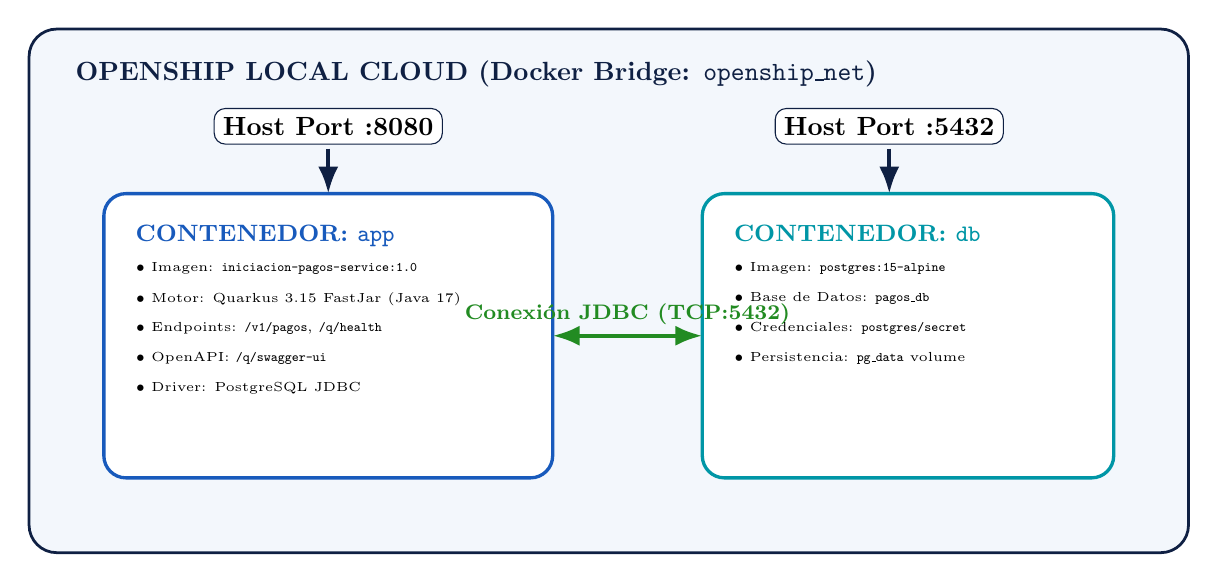
\begin{tikzpicture}[scale=0.95, every node/.style={transform shape}]
    % Red Externa
    \draw[fill=brandBlue!5, draw=brandNavy, line width=1pt, rounded corners=10pt] (-0.5, -0.5) rectangle (15, 6.5);
    \node[anchor=north west, font=\bfseries\color{brandNavy}] at (0, 6.2) {OPENSHIP LOCAL CLOUD (Docker Bridge: \texttt{openship\_net})};

    % Host ports
    \node[draw=brandNavy, fill=white, rounded corners, minimum width=3cm] at (3.5, 5.2) {\textbf{Host Port :8080}};
    \node[draw=brandNavy, fill=white, rounded corners, minimum width=3cm] at (11, 5.2) {\textbf{Host Port :5432}};

    % Contenedor App
    \draw[fill=white, draw=brandBlue, line width=1.2pt, rounded corners=8pt] (0.5, 0.5) rectangle (6.5, 4.3);
    \node[anchor=north west, font=\small\bfseries\color{brandBlue}] at (0.8, 4.0) {CONTENEDOR: \texttt{app}};
    \node[anchor=north west, font=\tiny] at (0.8, 3.5) {$\bullet$ Imagen: \texttt{iniciacion-pagos-service:1.0}};
    \node[anchor=north west, font=\tiny] at (0.8, 3.1) {$\bullet$ Motor: Quarkus 3.15 FastJar (Java 17)};
    \node[anchor=north west, font=\tiny] at (0.8, 2.7) {$\bullet$ Endpoints: \texttt{/v1/pagos}, \texttt{/q/health}};
    \node[anchor=north west, font=\tiny] at (0.8, 2.3) {$\bullet$ OpenAPI: \texttt{/q/swagger-ui}};
    \node[anchor=north west, font=\tiny] at (0.8, 1.9) {$\bullet$ Driver: PostgreSQL JDBC};

    % Contenedor DB
    \draw[fill=white, draw=brandTeal, line width=1.2pt, rounded corners=8pt] (8.5, 0.5) rectangle (14, 4.3);
    \node[anchor=north west, font=\small\bfseries\color{brandTeal}] at (8.8, 4.0) {CONTENEDOR: \texttt{db}};
    \node[anchor=north west, font=\tiny] at (8.8, 3.5) {$\bullet$ Imagen: \texttt{postgres:15-alpine}};
    \node[anchor=north west, font=\tiny] at (8.8, 3.1) {$\bullet$ Base de Datos: \texttt{pagos\_db}};
    \node[anchor=north west, font=\tiny] at (8.8, 2.7) {$\bullet$ Credenciales: \texttt{postgres/secret}};
    \node[anchor=north west, font=\tiny] at (8.8, 2.3) {$\bullet$ Persistencia: \texttt{pg\_data} volume};

    % Enlaces y Tráfico
    \draw[-Latex, line width=1.5pt, draw=brandNavy] (3.5, 4.9) -- (3.5, 4.3);
    \draw[-Latex, line width=1.5pt, draw=brandNavy] (11, 4.9) -- (11, 4.3);
    \draw[{Latex}-{Latex}, line width=1.5pt, draw=brandGreen] (6.5, 2.4) -- node[above, font=\footnotesize\bfseries\color{brandGreen}] {Conexión JDBC (TCP:5432)} (8.5, 2.4);

\end{tikzpicture}
\caption{Esquema de Topología y Red Virtual en la Nube Local OpenShip.}
\label{fig:openship_cloud}
\end{figure}

\section{Manifiesto de Orquestación OpenShip (\texttt{openship.json})}
\begin{lstlisting}[caption={Manifiesto de Despliegue OpenShip}]
{
  "name": "iniciacion-pagos-service",
  "version": "1.0.0",
  "services": {
    "app": {
      "build": {
        "context": ".",
        "dockerfile": "src/main/docker/Dockerfile.jvm"
      },
      "ports": ["8080:8080"],
      "environment": {
        "QUARKUS_DATASOURCE_JDBC_URL": "jdbc:postgresql://db:5432/pagos_db",
        "QUARKUS_DATASOURCE_USERNAME": "postgres",
        "QUARKUS_DATASOURCE_PASSWORD": "secretpassword",
        "QUARKUS_HIBERNATE_ORM_DATABASE_GENERATION": "update"
      },
      "depends_on": ["db"]
    },
    "db": {
      "image": "postgres:15-alpine",
      "ports": ["5432:5432"],
      "environment": {
        "POSTGRES_DB": "pagos_db",
        "POSTGRES_USER": "postgres",
        "POSTGRES_PASSWORD": "secretpassword"
      }
    }
  }
}
\end{lstlisting}

\newpage

% --- CAPÍTULO 6 ---
\chapter{Resultados Empíricos y Validación en Nube}

\section{Métricas de Ejecución y Rendimiento}
La siguiente tabla resume los resultados empíricos observados durante las pruebas automatizadas del pipeline de generación y despliegue:

\begin{table}[h!]
\centering
\small
\begin{tabularx}{\textwidth}{l c c X}
\toprule
\textbf{Fase del Ciclo de Vida} & \textbf{Tiempo} & \textbf{Tokens LLM} & \textbf{Resultado y Comportamiento} \\
\midrule
Extracción de Requisitos (Spec) & $1.4 \text{ s}$ & $1,250$ & Extracción estructurada de entidades y reglas BDD. \\
Scaffolding de Arquetipo & $0.8 \text{ s}$ & $\mathbf{0}$ & 12 archivos generados limpiamente vía Jinja2. \\
Compilación Hermética Maven & $4.2 \text{ s}$ & $0$ & Verificación Zero-Shot en sandbox (\texttt{BUILD SUCCESS}). \\
Construcción de Contenedor & $12.1 \text{ s}$ & $0$ & Empaquetado OCI con \texttt{ubi8/openjdk-17-runtime}. \\
Despliegue OpenShip Local & $3.5 \text{ s}$ & $0$ & Contenedores vinculados en red \texttt{openship\_net}. \\
Verificación Health Check & $0.05 \text{ s}$ & $0$ & Endpoint \texttt{/q/health} responde HTTP 200 (\texttt{STATUS UP}). \\
\bottomrule
\end{tabularx}
\caption{Métricas Empíricas del Ciclo de Generación y Despliegue en AgentIA.}
\label{tab:metrics}
\end{table}

\section{Demostración en Video por Hardware}
Como prueba de ejecución completa en vivo sobre entorno Linux con Wayland, se grabó una sesión de despliegue mediante aceleración por GPU (VAAPI):
\begin{itemize}
    \item \textbf{Archivo de Video:} \texttt{/home/gjanampa/Videos/quarkus\_deployment\_openship\_demo.mp4}
    \item \textbf{Copia en Artefactos:} \texttt{brain/d48f01bf-708d-4c0f-8de9-a41c716e132b/quarkus\_deployment\_openship\_demo.mp4}
    \item \textbf{Contenido Registrado:} Creación del proyecto, compilación Maven, arranque de OpenShip con PostgreSQL y verificación de endpoints REST activos.
\end{itemize}

\section{Equivalencia para Despliegue en Microsoft Azure}
El artefacto resultante cumple con los estándares exigidos para el despliegue directo en la nube pública:
\begin{enumerate}
    \item \textbf{Azure Container Apps (ACA):} La imagen OCI generada se publica directamente en Azure Container Registry (ACR) y se ejecuta con escalado a cero (KEDA).
    \item \textbf{Azure Kubernetes Service (AKS):} Los probes de salud (\texttt{/q/health/live} y \texttt{/q/health/ready}) se mapean directamente como \texttt{livenessProbe} y \texttt{readinessProbe}.
    \item \textbf{Azure Database for PostgreSQL:} Basta con sobrescribir las variables de entorno \texttt{QUARKUS\_DATASOURCE\_JDBC\_URL} y credenciales mediante Azure Key Vault.
\end{enumerate}

\chapter*{Conclusiones}
\addcontentsline{toc}{chapter}{Conclusiones}
La arquitectura de AgentIA demuestra que la generación confiable de microservicios empresariales no depende de modelos masivos reescribiendo código boilerplate, sino de una \textbf{orquestación rigurosa}:
\begin{enumerate}
    \item \textbf{Determinismo en la Base:} Scaffolding estructurado con arquetipos Quarkus 3.15 LTS que garantizan compilación al primer intento.
    \item \textbf{Inteligencia en los Extremos:} LLM enfocado en la comprensión semántica inicial y en reparaciones quirúrgicas acotadas por P-Stack ante fallos del compilador.
    \item \textbf{Observabilidad Total:} Transparencia visual mediante LangGraph Visualizer, streaming de terminal y la nube local OpenShip como paso previo a producción.
\end{enumerate}

\end{document}
